% Definiciones y constantes de estilo
% Clase del documento
\documentclass[a4paper,12pt,twoside,openright,titlepage]{book}

%
% Paquetes necesarios
%
\usepackage[T1]{fontenc}
\usepackage{pslatex}
% Símbolo del euro
\usepackage{eurosym}
% Codificación UTF8
\usepackage[utf8]{inputenc}
% Caracteres del español
\usepackage[spanish]{babel}
% Código, algoritmos, etc.
\usepackage{listings}
% Definición de colores
\usepackage{color}
% Extensión del paquete color
\usepackage[table,xcdraw]{xcolor}
% Márgenes
\usepackage{anysize}
% Cabecera y pie de página
\usepackage{fancyhdr}
% Estilo título tulos
\usepackage{quotchap}
% Algoritmos (expresarlos mejor)
\usepackage{algorithmic}
% Títulos de secciones
\usepackage{titlesec}
% Fórmulas matemáticas
\usepackage[cmex10]{amsmath}
% Enumeraciones
\usepackage{enumerate}
% Páginas en blanco
\usepackage{emptypage}
% Separación entre cajas
\usepackage{float}
% Imágenes
\usepackage[pdftex]{graphicx}
% Mejora de las tablas

\usepackage{array}
% Mejora de los símbolos matemáticos
\usepackage{mdwmath}
% Separar figuras en subfiguras
\usepackage[caption=false,font=footnotesize]{subfig}
% Incluir pdfs externos
\usepackage{pdfpages}
% Mejoras sobre las cajas
\usepackage{fancybox}
% Apéndices
\usepackage{appendix}
% Marcadores (para el pdf)
\usepackage{bookmark}
% Estilo de enumeraciones
\usepackage{enumitem}
% Espacio entre líneas y párrafos
\usepackage{setspace}
% Glosario/Acrónimos
\usepackage[acronym]{glossaries}
% Fuentes
\usepackage[T1]{fontenc}
% Bibliografía
\usepackage[sorting=none,natbib=true,backend=bibtex,bibencoding=ascii]{biblatex}
% Fix biblatex+babel warning
\usepackage{csquotes}
\usepackage{afterpage}
%Poner margenes al documento
\usepackage[centering, margin={2.54cm,2.54cm}, includeheadfoot]{geometry}




% Enlaces
\hypersetup{hidelinks,pageanchor=true,colorlinks,citecolor=Fuchsia,urlcolor=black,linkcolor=Cerulean}

%Capacidades matemáticas extra
\usepackage{amsmath} 
%librería de símbolos
\usepackage{amssymb}

% Euro (€)
\DeclareUnicodeCharacter{20AC}{\euro}

% Inclusión de gráficos
\graphicspath{{./graphics/}}

% Texto referencias
\addto{\captionsspanish}{\renewcommand{\bibname}{Bibliografía}}

% Extensiones de gráficos
\DeclareGraphicsExtensions{.pdf,.jpeg,.jpg,.png}

% Definiciones de colores (para hidelinks)
\definecolor{LightCyan}{rgb}{0,0,0}
\definecolor{Cerulean}{rgb}{0,0,0}
\definecolor{Fuchsia}{rgb}{0,0,0}

% Keywords (español e inglés)
\def\keywordsEn{\vspace{.5em}
{\textbf{\textit{Key words ---}}\,\relax%
}}
\def\endkeywordsEn{\par}

\def\keywordsEs{\vspace{.5em}
{\textbf{\textit{Palabras clave ---}}\,\relax%
}}
\def\endkeywordsEs{\par}


% Abstract (español e inglés)
\def\abstractEs{\vspace{.5em}
{\textbf{\textit{Resumen ---}}\,\relax%
}}
\def\endabstractEs{\par}

\def\abstractEn{\vspace{.5em}
{\textbf{\textit{Abstract ---}}\,\relax%
}}
\def\endabstractEn{\par}

% Estilo páginas de capítulos
\fancypagestyle{plain}{
\fancyhf{}
\fancyfoot[CO]{\footnotesize\emph{\nombretrabajo}}
\fancyfoot[RO]{\vspace{0.4cm}\thepage}
\renewcommand{\footrulewidth}{.6pt}
\renewcommand{\headrulewidth}{0.0pt}
}

% Estilo resto de páginas
\pagestyle{fancy}

% Estilo páginas impares
\fancyfoot[CO]{\footnotesize\emph{\nombretrabajo}}
\fancyfoot[RO]{\vspace{0.4cm}\thepage}
%\fancyfoot[LO]{
\includegraphics[width=.08\textwidth]{escudo}}

\rhead[]{\leftmark}


% Estilo páginas pares
\fancyfoot[CE]{\emph{\pieparcen}}
\fancyfoot[LE]{\vspace{0.4cm}\thepage}
%\fancyfoot[RE]{
\includegraphics[width=.08\textwidth]{escudo}}
\lhead[\leftmark]{}


% Guía del pie de página
\renewcommand{\footrulewidth}{.6pt}

% Nombre de los bloques de código
\renewcommand{\lstlistingname}{Código}

% Estilo de los lstlistings
\lstset{
    frame=tb,
    breaklines=true,
    postbreak=\raisebox{0ex}[0ex][0ex]{\ensuremath{\color{gray}\hookrightarrow\space}}
}

% Definiciones de funciones para los títulos
\newlength\salto
\setlength{\salto}{3.5ex plus 1ex minus .2ex}
\newlength\resalto
\setlength{\resalto}{2.3ex plus.2ex}

% Estilo de los acrónimos
\renewcommand{\acronymname}{Glosario}
\renewcommand{\glossaryname}{Glosario}
\pretolerance=2000
\tolerance=3000

% Texto índice de tablas
\addto\captionsspanish{
\def\tablename{Tabla}
\def\listtablename{\'Indice de tablas}
}

% Traducir appendix/appendices
\renewcommand\appendixtocname{Anexos}
\renewcommand\appendixpagename{Anexos}

% Comando code (lstlisting sin cambio de página)
\lstnewenvironment{code}[1][]%
  { \noindent\minipage{0.935\linewidth}\medskip
    \vspace{5mm}
    \lstset{basicstyle=\ttfamily\footnotesize,#1}}
  {\endminipage}
  
% Colores

\definecolor{rositaoscuro}{RGB}{219, 0, 122}


% Definiciones de comandos
\newcommand{\nombreautor}{Miriam Rubio Lecuona}
\newcommand{\nombretrabajo}{Prácticas curriculares en Movalsys S.L.}
\newcommand{\fecha}{Mayo de 2019}
\newcommand{\grado}{TODO: Grado}

\newcommand{\universidad}{Universidad Pública de Navarra}
\newcommand{\pieparizq}{TODO: Pie de página par}
\newcommand{\pieparcen}{Prácticas curriculares en Movalsys S.L}
\newcommand{\logo}{graphics/logo_movalsys}


% Inicio del documento
\begin{document}

% Elección del idioma (español)
\selectlanguage{spanish}

%
% Portada
%
\pagenumbering{gobble}
%
% Portada
%


\includepdf{cover.pdf}
% Primera página
\pagenumbering{Alph}
\thispagestyle{empty}

\begin{flushleft}
	\begin{scriptsize}
	\end{scriptsize}\end{flushleft}

	\thispagestyle{empty}
	\begin{center}
		
		% Nombre del trabajo
		\textbf{\begin{large}
				\MakeUppercase{\nombretrabajo}\\*
			\end{large}}
			\vspace*{2cm}
			\begin{figure}[H]
				\centering
				
\includegraphics[]{escudo}
			
			\end{figure}
			\vspace{3cm}
			
			% Nombre del autor y del tutor
			\large Autora: \nombreautor \\*
			\large Tutoras: \nombretutor \\*
			\vspace*{1.5cm}
					
			\departamento \\
%			\facultad \\
			\universidad \\
			\vspace{1cm}
			\fecha \\
			
			\clearpage
			
		\end{center}
		\normalsize

\hypersetup{pageanchor=true}

% Estilo de párrafo de los capítulos
\setlength{\parskip}{0.75em}
\renewcommand{\baselinestretch}{1.25}
% Interlineado simple
\spacing{1.5}



% Estilo de párrafo de los índices
\setlength{\parskip}{1pt}
\renewcommand{\baselinestretch}{1}

%
% Tabla de contenidos
%
\tableofcontents
\cleardoublepage

% Estilo de párrafo de los capítulos
\setlength{\parskip}{0.75em}
\renewcommand{\baselinestretch}{1.25}
% Interlineado 1.5
\spacing{1.5}
% Numeración contenido
\pagenumbering{arabic}
\setcounter{page}{1}



%
% Introducción
%

\chapter{Sobre la empresa}

	\section{Historia de Movalsys S.L}
		Movalsys es una empresa que se constituye en diciembre de 2015 y que surge de la experiencia investigadora de dos grupos de investigación (Álgebra y Aplicaciones y Biomecánica y Fisiología del movimiento (BIOFIM)) de la Universidad Pública de Navarra. 
		
		Movalsys S.L. desarrolla y comercializa tecnología para la medición rápida y sencilla de los parámetros biomecánicos que caracterizan el movimiento humano. Esta tecnología no se limita a la mera obtención de dichos parámetros, sino que se apoya en el conocimiento reunido durante diez años por investigadores de Universidad Pública de Navarra para contextualizarlos y ofrecer una
		interpretación simple y directa del estado físico del sujeto y de su rendimiento.
		El objetivo de Movalsys es ofrecer a los profesionales de la salud herramientas que les sirvan de apoyo en el diagnóstico, el seguimiento y la óptima recuperación de sus pacientes, facilitándoles el acceso a la valoración biomecánica del movimiento humano.
	
	
	\section{Dedicación de la empresa}
	 
	Este equipo multidisciplinar lleva ocho años realizando investigaciones sobre el análisis de señales biomecánicas proporcionadas por sensores inerciales y sus avances han sido publicados en importantes revistas científicas en Fisioterapia, Geriatría, Ingeniería y Matemáticas.
	
	La dedicación de la empresa consiste fundamentalmente en la obtención y procesado de parámetros mediante sensores inerciales, es decir, en el análisis del movimiento. Por tanto su campo de aplicación puede ser tanto la práctica deportiva (mejora de rendimiento, prevención de lesiones), como el de la rehabilitación (riesgo de caídas, fragilidad,etc.). Actualmente se está explorando el campo de la neuro-rehabilitación y de la prevención de riesgos laborales en las industrias (ver figura \ref{mercado}). 
	 \begin{figure}[H]
	 	\centering
	 	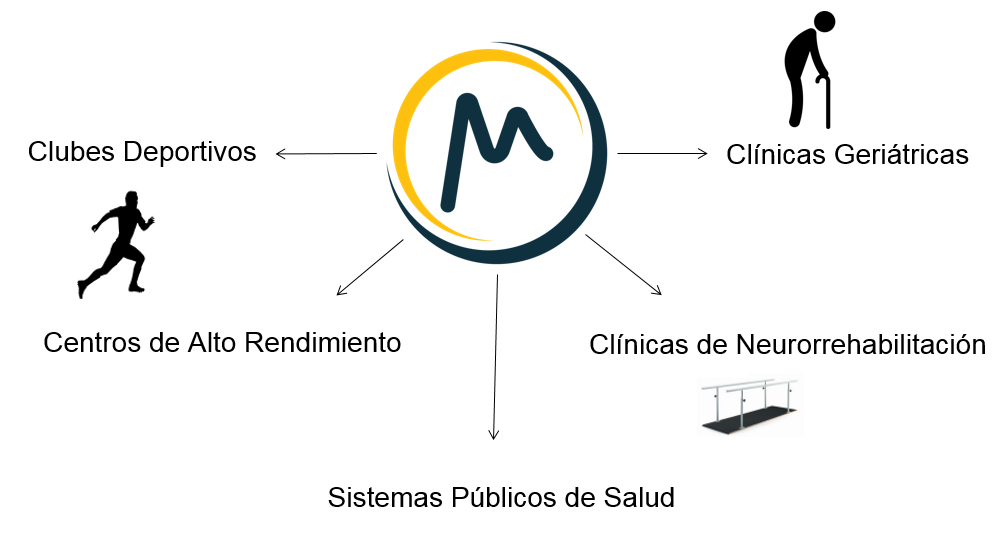
\includegraphics[width=0.8\textwidth]{./graphics/mercado}\label{mercado}
	 	
	 \end{figure}
	\section{Estructura de la empresa} \label{empresa}
	

		Movalsys S.L. es una sociedad limitada en la que todos sus trabajadores son socios de la misma y además cuentan con colaboración externa para el desarrollo de su actividad.
		
		A continuación se describen los roles de cada uno de los mismos:
		\begin{itemize}
			\item \textbf{Mariano Velasco}: Director gerente. Su objetivo es principalmente el de reunirse con miembros de otras empresas para conseguir proyectos. Es la imagen pública de la empresa. Su dedicación es principalmente la de la gestión de la empresa. Se encarga tanto de la coordinación del equipo como de la burocracia. Además, es el principal encargado de reunirse con diferentes clientes así como de realizar la promoción de la empresa en diferentes eventos.
			 \begin{figure}[H]
			 	\centering
			 	
\includegraphics[width=0.25\textwidth]{./graphics/mariano}

			 \end{figure}
			\item \textbf{Pablo Lecumberri}: Es el ingeniero de software, encargado del software de medición que utiliza la empresa. Se trata de un empleado de carácter técnico que resulta fundamental especialmente en las reuniones con clientes.
			\begin{figure}[H]
				\centering
				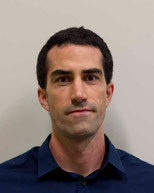
\includegraphics[width=0.25\textwidth]{./graphics/pablo}
				
			\end{figure}
			\item \textbf{Marisol Gómez}: directora de investigación. Se encarga de la búsqueda de ayudas de investigación y de buscar nuevas áreas de desarrollo de la empresa. Actualmente su actividad está centrada en la neuro-rehabilitación.
			\begin{figure}[H]
				\centering
				
\includegraphics[width=0.25\textwidth]{./graphics/marisol}
				
			\end{figure}
			\item \textbf{Alicia Martínez}: Responsable de ventas. Se encarga de la gestión de facturas así como de la búsqueda de nuevos clientes. 
			\begin{figure}[H]
				\centering
				
\includegraphics[width=0.25\textwidth]{./graphics/alicia}
				
			\end{figure}
			\item \textbf{Nora Millor}: Responsable de atención al cliente. Es al encargada de estar en contacto con clientes, realizar un seguimiento de funcionamiento del sistema y de 
			\begin{figure}[H]
				\centering
				
\includegraphics[width=0.25\textwidth]{./graphics/nora}
				
			\end{figure}
			\item \textbf{Mikel Izquierdo}: es catedrático y director del departamento de Ciencias de la Salud. Se trata de un profesional muy reconocido en el campo de la salud y por ello también actúa como asesor y se dedica además a la búsqueda de contactos, lo cual en esta etapa de la empresa resulta imprescindible.
			\begin{figure}[H]
				\centering
				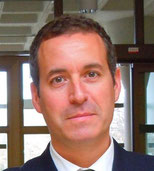
\includegraphics[width=0.25\textwidth]{./graphics/mikel}
				
			\end{figure}
			\item \textbf{Igor Setuain}: colaborador externo. Es doctor en fisioterapia y asesora a la empresa sobre los parámetros obtenidos en las mediciones dándoles sentido clínico.
			
		\end{itemize}
		
	Además de sus funciones principales, Pablo, Marisol, Nora, Alicia y Mariano se encargan de hacer el análisis de señales y de las mediciones. No participan todos siempre puesto que depende de la carga de trabajo de cada uno.
	
	Con respecto a la jerarquía de la empresa puede decirse que es plana, es decir, a pesar de existir la figura de director gerente, las decisiones se realizan de forma que todos los socios participan en ella. Se discuten en las reuniones semanales. El hecho de que cada empleado sienta responsabilidad en la toma de decisiones hace que se sientan integrados y valorados en la empresa, por tanto, que crezca su motivación y, además obtener diferentes perspectivas sobre un tema que permiten que las decisiones se enriquezcan. Además el hecho de que sean socios de la empresa provoca un sentimiento de responsabilidad en la misma, ya que la empresa es suya.
		


	\section{Plan estratégico}
	
	El plan estratégico es un programa de actuación que consiste en aclarar lo que pretendemos conseguir y cómo nos proponemos conseguirlo. Debido a que se trata de una start-up, no existe un plan estratégico claro ya que precisamente lo que caracteriza a este tipo de empresas es que se encuentran en fase de búsqueda de un modelo de negocio beneficioso para ellas.
		
		Actualmente uno de los trabajos que se desarrollan en la empresa es la búsqueda de producto y clientes/proyectos y mediante dicho trabajo se pretende buscar una solución para el plan estratégico de la empresa. Las decisiones se toman según aparezcan clientes, pero la definición clara de cómo actuar ante ciertas propuestas o qué productos ofrecer no está cerrada del todo debido a que todavía es necesaria la evaluación de las posibilidades que ofrece la empresa y cuáles de estas resultan más beneficiosas.
		
		
	
	\section{Funcionamiento general}
	
	El funcionamiento de la empresa es simple debido al reducido tamaño de la misma (5 empleados + 1 becaria). Cada uno de los componentes tiene claro el rol que desempeña en la empresa.
	
	La semana se compone generalmente de reuniones con clientes para buscar nuevos proyectos y de desarrollar aquellos que están en marcha, es decir, realizar análisis de los datos medidos y los informes oportunos. Además cada miembro desarrolla en paralelo cada una de las funciones de la cual es responsable (apartado \ref{empresa}).
	
	Debido al buen ambiente de trabajo ya que se conocen desde hace varios años, la motivación es alta. Además, a esto se le suma el que los miembros son socios por lo que tienen una motivación adicional por que todo salga bien. 
	
	Con respecto a retención de personal, están interesados en que llegue el día en el que puedan contratar a gente para repartir carga de trabajo. En mi caso, han estado enseñándome continuamente lo que hacen en la empresa y me han enseñado a realizar algunos de los análisis que llevan a cabo. Además, cuentan conmigo para un proyecto futuro relacionado con la temática de mi Trabajo Fin de Máster. Están dispuestos a dar oportunidad a gente nueva y a que la empresa crezca. Han ido guiando mi participación en las actividades con mucho interés e intentando integrar mi trabajo en el día a día de la empresa lo que ha hecho que mi interés y motivación en la empresa crezcan.
	
	

% Estado del arte
%
\chapter{Mi experiencia en la empresa}

	\section{Actividades}
	
		Durante la experiencia en la empresa he participado en diferentes actividades, partiendo de aquellas que únicamente requieren de observación y evolucionando hacia aquellas en las que he tomado parte activamente.
	
		\subsection{Reuniones}
		
				
			Existen dos tipos de reuniones en Movalsys, las semanales y las concertadas con clientes. Todas ellas son muy diferentes puesto que los objetivos son totalmente distintos. En las primeras de ellas, el objetivo fundamental es la actualización de los proyectos y las segundas pretenden buscar mercado y negocio.
			 
			En cuanto a las reuniones semanales realizadas en la empresa, he participado en todas ellas, ya que en ocasiones éstas coincidían con alguna actividad, visita o reunión en otra parte. Las reuniones se basaban en una mera puesta al día de los proyectos en los que la empresa está trabajando.
			
			Todas estas reuniones han seguido el mismo patrón aproximadamente. Mariano, el gerente, expone los puntos que tiene para comentar. Explica las novedades de cada uno de ellos, y los miembros del resto del equipo que intervienen en el proyecto en cuestión participan.
			
			Debido a que se trata de una empresa de reciente creación, las reuniones se dividen en dos partes fundamentales, que son:
			\begin{itemize}
				\item Estrategias empresariales.
				\item Datos técnicos de los proyectos.
			\end{itemize}
			
			Dependiendo de evento más próximo que tenga la empresa, es decir, según si el siguiente paso es el de realizar alguna presentación en alguna empresa o casos similares, las reuniones toman mayor aspecto técnico o no.
			
			Evaluando ahora las reuniones con posibles clientes, aunque en ellas he intervenido la mayoría de las ocasiones de forma pasiva, he observado notables diferencias con respecto a las reuniones internas de la empresa. En ellas se observa claramente la estrategia de negocio que se ha decidido en las reuniones y se ven las distintas posiciones de ambas partes. Después de éstas reuniones, se realiza una valoración entre los miembros asistentes a la misma en las que se proponen diferentes estrategias para poder conseguir el cliente, o colaborador, etc. Estas son las reuniones en las que quizá se aprende más sobre el mundo empresarial o quizás las más nuevas para mí.
			
			A veces, es cierto, que surgen reuniones esporádicas que suelen resolverse a la hora del descanso de la mañana. Suelen tener como objetivo comentar algún aspecto técnico puntual, o bien la propuesta de alguna reunión o el cuadrar horarios con el compañero con el que se está desarrollando alguno de los proyectos,etc. Éstas resultan más informales y no es necesario reunir a todos los miembros del equipo para ello.
			
		\subsection{Tareas}
					
			A lo largo del período de prácticas en la empresa las actividades han ido variando desde aquellas más sencillas a aquellas con mayor carga de responsabilidad. Puede dividirse en tres sub-períodos:
			
				\begin{enumerate}
					\item \textbf{Mediados de Febrero - Mediados de Marzo}.
					
					 Se trata de una etapa de observación y de aprendizaje de los procesos de medida mediante la asistencia a los mismos. Por ejemplo: medida realizada en el parque de bomberos de Cordovilla.
					
					También se realiza una visita a Adacen (Asociación de daño cerebral de Navarra) con el fin de asesorar técnicamente a los fisioterapeutas sobre un producto de rehabilitación motora que vino a ofrecer la empresa Vitia de San Sebastián. 
					
					\item \textbf{Mediados de Marzo - Mediados de Abril}.
					
					En esta ocasión se realiza un reparto de tareas en la que se me encarga la búsqueda de un sistema de sujeción de unos sensores para la práctica deportiva. El objetivo de la misma era tenerlo para la reunión semanal de la semana siguiente donde debía exponer mis progresos. Esto sirvió para empezar a sentirme parte de la empresa y empezar a tomar responsabilidades.
					
					Además, en este período asisto a unas jornadas en CEIN en las cuales varias empresas, entre ellas Movalsys, realizan propuestas a la empresa KyB. Movalsys realiza la propuesta en relación a prevención de riesgos laborales. Acabadas las exposiciones, nos reunimos con el directivo encargado de esa sección y se consigue llegar a un acuerdo para realizar un estudio en su empresa.
					
					Por último, se me encarga también la redacción de la parte de memoria técnica de una solicitud de proyecto de I+D+I del Gobierno de Navarra. En ella debía incluir la parte técnica relacionada con el TFM así como integrar otros sistemas ya que se trataba de un proyecto de transferencia de conocimiento. En este caso, el aprendizaje se centró más en temas burocráticos que no conocía hasta el momento.
						
					\item \textbf{Mediados de Abril - Mediados de Mayo}.
					
					Aproximadamente durante un mes que empezó en Abril, Movalsys ha estado realizando medidas en la Volkswagen. Una vez realizadas las medidas había que analizar las señales recogidas. En este caso, se me propone el  participar en este proyecto. A partir de este momento, las actividades que realizo empiezan a tomar relevancia ya que es el  trabajo que también realiza el resto del equipo.
					
					Además de la participación en este proyecto ya iniciado, realizamos una visita a la fábrica de KyB en los Arcos para observar los distintos puestos de trabajo y poder realizar la propuesta de ergonomía a la empresa para poder mejorar el aspecto de las lesiones de los trabajadores. Se pretende realizar un estudio parecido al realizado en Volkswagen.
					
					\item \textbf{Mediados de Mayo - Fin de la práctica}.
					
					En este último mes se ha centrado más en la redacción de memorias y en realizar medidas relacionadas con el TFM. Esto se ha compaginado con la elaboración de un informe general que se quiere diseñar en la empresa para la presentación de datos a los clientes y con la preparación de unos folletos para un encuentro de empresas en Bidart (Francia). También he participado en las decisiones.
					
				\end{enumerate}		
		
Además de todo ello, he participado en la corrección de propuestas, o consulta de ciertos temas de la empresa que normalmente se realizan por correo electrónico.
			
	\section{Problemas y soluciones}
	
Los principales problemas en los que se ha visto inmerso la empresa es en la búsqueda de financiación debido a que es una empresa de reciente creación. En este caso se busco una consultora con la que actualmente trabajan para la ayuda de Instrumento PyME. Se valoraron varias consultoras hasta encontrar la que más se adaptaba a las condiciones de Movalsys.

Otro de los problemas cotidianos de la empresa es el saber cuándo rechazar o aceptar ofertas ya que por una parte, tienen la necesidad de aceptar proyecto pero por otra parte, deben ofrecer algún tipo de beneficio tanto económico como para dar a conocer la empresa. Durante mi estancia en las prácticas surgió el caso de realizar un proyecto de colaboración con un centro tecnológico en Navarra y se planteó el poder llevarlo a cabo. Cuando realizaron la propuesta, cada uno de nosotros la recibió por e-mail con el fin de poder estudiarla. En una reunión semanal cada uno opinó y se rechazó la propuesta debido a que la cantidad de dinero que se pedía en un principio excedía lo que la empresa estaba dispuesta a poner. Por ello, se busco otra alternativa, que fue la de la consultora anteriormente mencionada.

Todo este tipo de contratiempos/decisiones se toman entre todos los miembros. Es la ventaja de tratarse de una empresa pequeña. Todas las opiniones tienen cabida y se pueden debatir.

	
	
	\section{Recursos materiales}

Los recursos materiales de los que dispone la empresa son adecuados a sus necesidades.
Gracias a que han ganado premios de emprendimiento disponen de sede en CEIN y debido a que es una empresa Spin-off de la UPNA dispone de ordenadores y un laboratorio donde también puede desarrollar su actividad. Además, ha conseguido un laboratorio en NavarraBioMed donde a partir de Junio va a llevar parte de su actividad.

Realmente no es una empresa que precise de muchos recursos materiales. Únicamente necesita los sensores para la medición y equipo informático donde analizar las señales y llevar a cabo el desarrollo del software.
	
	


%
% Conclusiones
%
\chapter{Conclusiones y líneas futuras\label{sec:conclusiones}}


%Este ejercicio resulta verdaderamente beneficioso en el aprendizaje. 


Los resultados de este trabajo han sido útiles para determinar la viabilidad al realizar un primer prototipo como solución al problema planteado. El comparar dos tecnologías diferentes para una misma aplicación permite entender en mayor magnitud las posibilidades de cada una de las tecnologías. 


%Este ha sido un trabajo muy completo al tomar tanto en cuenta ejercicio de desarrollo software como hardware. 

Durante la realización del prototipo basado en redes de difracción de Bragg se han encontrado diversas dificultades:

\begin{itemize}
	\item \textbf{Tecnología muy delicada.} La fibra del sensor FBG es muy delicada para el proceso de fabricación del guante y las herramientas disponibles en el laboratorio. 
	Tanto en el proceso de fabricación como en la posterior manipulación la fragilidad de las fibras hace prácticamente imposible su futuro uso como sensor de movimiento para esta aplicación.
	%Pese haber tenido mucho cuidado a la hora de manipularla ha sido imposible evitar que se rompiera en múltiples ocasiones. Además una vez el prototipo ha sido fabricado con éxito, sin que se rompa ninguna fibra, estas siguen siendo susceptibles de romperse. Por ello no es la mejor tecnología para medir movimientos continuados, que rompen la fibra pese a estar embebida en PDMS. 
	 
	\item \textbf{Diseño del guante no apto para todas las manos.} El diseño del guante no es apropiado para la finalidad inicial del prototito. %Al no ser posible colocar siempre el guante en la misma posición sobre la mano, las medidas obtenidas de una misma posición en diferentes ocasiones son diferentes. Mucho más aún cuando se colocan en manos con diferente fisionomía. 
	%, lo que dificulta la caracterización del movimiento respecto al comportamiento de los sensores. 
	Se trata de un condicionamiento importante. Para conseguir caracterizar el comportamiento de las FBGs con los ángulos de apertura es necesario que siempre se coloque el guante de tal forma que el vértice del ángulo coincida en el mismo punto. La forma de las diferentes manos de las personas hace que no sea posible una caracterización como la citada. Unicamente puede ser útil para evaluar el rango de movimiento y velocidad dentro de una misma sesión de rehabilitación. Aunque se pierda la información frente a una referencia global del movimiento, sigue ofreciendo al usuario una experiencia satisfactoria pese a no cumplir con la plenitud de los objetivos marcados.
	
	Para medir en cualquier tipo de mano con una referencia global, el diseño sería mucho más complejo. Haría falta buscar la manera de se pudiera colocar cada dedo independientemente para ajustar la posición del vértice del ángulo a medir y reforzar el recubrimiento de los sensores impidiendo que se dieran las deformaciones que la fibra no sea capaz de soportar.
	
	
	
	\item \textbf{Software no escalable.} Pese a ser LabVIEW un lenguaje cuya programación es muy visual, cuando se trata de partir de un proyecto desarrollado, como es el caso del software del interrrogador, resulta bastante tedioso adaptar el nuevo programa.
	
	Además la experiencia de usuario se ve muy limitada ya que LabVIEW no es muy configurable en la parte de front-end.
	
	Otro contratiempo importante del software son los problemas que da al iniciarlo. Al iniciar el software del interrogador saltan alertas de error en la señal que no permiten seguir con la ejecución. Durante el desarrollo del proyecto se ha conseguido intuir el procedimiento en el que dichas alertas saltan con menos frecuencia y de ello surgen ciertos pasos del protocolo de medida.  %-viene de fbg- 
	 
	
	 
\end{itemize}

\clearpage

Se concluye el trabajo descartando la tecnología de sensores de FBG para la evaluación de la rehabilitación de las manos. Siendo esto motivado por no cumplir con las expectativas funcionales requeridas, además de por la complejidad de su manufacturación y su delicadeza. 

Se ha propuesto un diseño que cumplirá con las expectativas de medir el movimiento de las manos, obteniendo datos comparables entre sesiones. La solución planteada presta especial atención las especificaciones que el prototipo de FBG no ha cumplido. Ofrecerá mayor versatilidad y capacidad para añadir nuevas funcionalidades. Los sensores inerciales permitirán comunicación inalámbrica, robustez del diseño y bajo precio.








\section{Líneas futuras}

A partir de la experiencia del desarrollo de este proyecto se realizará el guante basado en sensores inerciales propuesto en la memoria.

\begin{itemize}
	\item El desarrollo del guante sensorizado se realizará siguiendo un proceso modular. Se dividirá el escenario global en varios escenarios, simplificando así su realización. Añadiendo las funcionalidades de cada dedo progresivamente, comenzando por el pulgar y el índice. 
	 
	\item En paralelo a este desarrollo se realizará el desarrollo del software por su dependencia, dejando para el final el desarrollo grueso de las funcionalidades más allá de la interpretación de las medidas de los sensores. 
	
	%La aplicación se programará en C++, siendo más adaptable a las necesidades de programación. Así el desarrollador tiene más facultad a la hora de programar. 
	 
	\item La aplicación se programará en C++, debido a que tiene una extensa documentación y es mas moldeable segun nuestras necesidades.
	
	\item Debido al contexto en el que se aplica el sistema, se debe tener en cuenta la ergonomía del mismo, la autonomía y el coste.
	Asimismo deberá cumplir con unas especificaciones óptimas para poder obtener resultados fiables. Sería recomendable contar con la experiencia de in ingeniero de diseño que paralelamente, con el desarrollo electrónico, procesado de señal y comunicaciones, se centre en el ámbito del diseño y la ergonomía del dispositivo.
	
	
	%Este diseño tiene capacidad para abarcar más funcionalidades de las propuestas. El desarrollo de estas no corresponde a esta memoria, pero merecen mención en este apartado para comprender mejor el alcance de esta tecnología. 
	
	\item El guante contará con capacidad inalámbrica, haciendo su uso mucho más cómodo al aportarle portabilidad.
	
	\item Una posibilidad más que ofrece el guante es añadirle funcionalidad actuadora para acompañar a los pacientes en el movimiento de las manos durante sus ejercicios de rehabilitación. 
\end{itemize} 




% No expandir elementos para llenar toda la página
\raggedbottom




% Fin del documento
\end{document}
